\section*{Introduction}

PBMath is a C library providing mathematical structures and functions.\\ 

The \begin{ttfamily}VecFloat\end{ttfamily} structure and its functions can be used to manipulate vectors of float values.\\

The \begin{ttfamily}VecShort\end{ttfamily} structure and its functions can be used to manipulate vectors of short values.\\

The \begin{ttfamily}MatFloat\end{ttfamily} structure and its functions can be used to manipulate matrices of float values.\\

The \begin{ttfamily}Gauss\end{ttfamily} structure and its functions can be used to get values of the Gauss function and random values distributed accordingly with a Gauss distribution.\\

The \begin{ttfamily}Smoother\end{ttfamily} functions can be used to get values of the SmoothStep and SmootherStep functions.\\

The \begin{ttfamily}EqLinSys\end{ttfamily} structure and its functions can be used to solve systems of linear equation.\\

It uses the \begin{ttfamily}PBErr\end{ttfamily} library.\\

\section{Definitions}

\subsection{Vector}

\subsubsection{Distance between two vectors}

For \begin{ttfamily}VecShort\end{ttfamily}:\\

\begin{equation}
\begin{array}{l}
Dist(\overrightarrow{v},\overrightarrow{w})=\sum_i|v_i-w_i|\\
HamiltonDist(\overrightarrow{v},\overrightarrow{w})=\sum_i|v_i-w_i|\\
PixelDist(\overrightarrow{v},\overrightarrow{w})=\sum_i|v_i-w_i|\\
\end{array}
\end{equation}
For \begin{ttfamily}VecFloat\end{ttfamily}:\\
\begin{equation}
\begin{array}{l}
Dist(\overrightarrow{v},\overrightarrow{w})=\sum_i(v_i-w_i)^2\\
HamiltonDist(\overrightarrow{v},\overrightarrow{w})=\sum_i|v_i-w_i|\\
PixelDist(\overrightarrow{v},\overrightarrow{w})=\sum_i\left|\lfloor v_i\rfloor -\lfloor w_i\rfloor\right|\\
\end{array}
\end{equation}

\subsubsection{Angle between two vectors}

The problem is as follow: given two vectors $\vec{V}$ and $\vec{W}$ not null, how to calculate the angle $\theta$ from $\vec{V}$ to $\vec{W}$.\\

Let's call $M$ the rotation matrix: $M\vec{V}=\vec{W}$, and the components of $M$ as follow:
\begin{equation}
M=\left[
\begin{array}{cc}
Ma&Mb\\
Mc&Md\\
\end{array}
\right]=\left[
\begin{array}{cc}
cos(\theta)&-sin(\theta)\\
sin(\theta)&cos(\theta)\\
\end{array}
\right]
\end{equation}
Then, $M\vec{V}=\vec{W}$ can be written has 
\begin{equation}
\left\lbrace
\begin{array}{l}
W_x = M_aV_x+M_bV_y\\
W_y = M_cV_x+M_dV_y\\
\end{array}
\right.
\end{equation}
Equivalent to
\begin{equation}
\left\lbrace
\begin{array}{l}
W_x = M_aV_x+M_bV_y\\
W_y = -M_bV_x+M_aV_y\\
\end{array}
\right.
\end{equation}
where $M_a=cos(\theta)$ and $M_b=-sin(\theta)$.\\
If $Vx\neq0.0$, we can write
\begin{equation}
\left\lbrace
\begin{array}{l}
M_b = \frac{M_aV_y-W_y}{V_x}\\
M_a = \frac{W_x+W_yV_y/V_x}{V_x+V_y^2/V_x}\\
\end{array}
\right.
\end{equation}
Or, if $Vx=0.0$, we can write
\begin{equation}
\left\lbrace
\begin{array}{l}
Ma = \frac{W_y+M_bV_x}{V_y}\\
Mb = \frac{W_x-W_yV_x/V_y}{V_y+V_x^2/V_y}\\
\end{array}
\right.
\end{equation}
Then we have $\theta=\pm cos^{-1}(M_a)$ where the sign can be determined by verifying that the sign of $sin(\theta)$ matches the sign of $-M_b$: if $sin(cos^{-1}(M_a))*M_b > 0.0$ then multiply $\theta=-cos^{-1}(M_a)$ else $\theta=cos^{-1}(M_a)$.

\subsection{Matrix}

\subsubsection{Inverse matrix}

The inverse of a matrix is only implemented for square matrices less than 3x3. It is computed directly, based on the determinant and the adjoint matrix.\\

For a 2x2 matrix $M$:\\

\begin{equation}
M^{-1}=\frac{1}{det}\left[\begin{array}{cc}
M_3&-M_2\\
-M_1&M_0\\
\end{array}\right]
\end{equation}
where
\begin{equation}
M=\left[\begin{array}{cc}
M_0&M_2\\
M_1&M_3\\
\end{array}\right]
\end{equation}
and
\begin{equation}
det=M_0M_3-M_1M_2
\end{equation}

For a 3x3 matrix $M$:\\

\begin{equation}
M^{-1}=\frac{1}{det}\left[\begin{array}{ccc}
(M_4M_8-M_5M_7)&-(M_3M_8-M_5M_6)&(M_3M_7-M_4M_6)\\
-(M_1M_8-M_2M_7)&(M_0M_8-M_2M_6)&-(M_0M_7-M_1M_6)\\
(M_1M_5-M_2M_4)&-(M_0M_5-M_2M_3)&(M_0M_4-M_1M_3)\\
\end{array}\right]
\end{equation}
where
\begin{equation}
M=\left[\begin{array}{ccc}
M_0&M_3&M_6\\
M_1&M_4&M_7\\
M_2&M_5&M_8\\
\end{array}\right]
\end{equation}
and
\begin{equation}
\begin{array}{ll}
det=&M_0(M_4M_8-M_5M_7)-\\
&M_3(M_1M_8-M_2M_7)+\\
&M_6(M_1M_5-M_2M_4)\\
\end{array}
\end{equation}

\section{Interface}

\begin{scriptsize}
\begin{ttfamily}
\verbatiminput{../pbmath.h}
\end{ttfamily}
\end{scriptsize}

\section{Code}

\subsection{pbmath.c}

\begin{scriptsize}
\begin{ttfamily}
\verbatiminput{../pbmath.c}
\end{ttfamily}
\end{scriptsize}

\subsection{pbmath-inline.c}

\begin{scriptsize}
\begin{ttfamily}
\verbatiminput{../pbmath-inline.c}
\end{ttfamily}
\end{scriptsize}

\section{Makefile}

\begin{scriptsize}
\begin{ttfamily}
\verbatiminput{../Makefile}
\end{ttfamily}
\end{scriptsize}

\section{Unit tests}

\begin{scriptsize}
\begin{ttfamily}
\verbatiminput{../main.c}
\end{ttfamily}
\end{scriptsize}

\section{Unit tests output}

\begin{scriptsize}
\begin{ttfamily}
\verbatiminput{../unitTestRef.txt}
\end{ttfamily}
\end{scriptsize}

\section{Examples}

vecshort.txt:\\
\begin{scriptsize}
\begin{ttfamily}
\verbatiminput{../vecshort.txt}
\end{ttfamily}
\end{scriptsize}

vecfloat.txt:\\
\begin{scriptsize}
\begin{ttfamily}
\verbatiminput{../vecfloat.txt}
\end{ttfamily}
\end{scriptsize}

matfloat.txt:\\
\begin{scriptsize}
\begin{ttfamily}
\verbatiminput{../matfloat.txt}
\end{ttfamily}
\end{scriptsize}

smoother functions:\\
\begin{center}
\begin{figure}[H]
\centering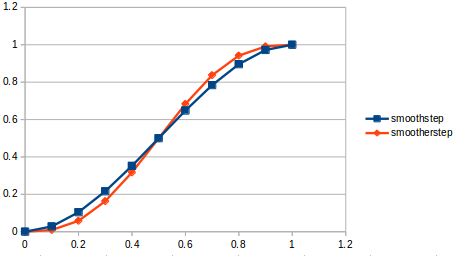
\includegraphics[width=6cm]{./smoother.png}\\
\end{figure}
\end{center}

gauss function (mean:0.0, sigma:1.0):\\
\begin{center}
\begin{figure}[H]
\centering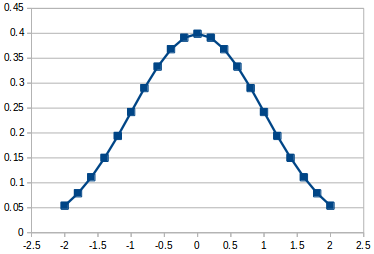
\includegraphics[width=6cm]{./gauss.png}\\
\end{figure}
\end{center}

gauss rand function (mean:1.0, sigma:0.5):\\
\begin{center}
\begin{figure}[H]
\centering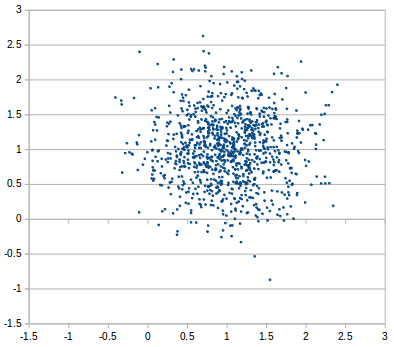
\includegraphics[width=6cm]{./gaussrnd.png}\\
\end{figure}
\end{center}

